\documentclass[a4paper,11pt,twoside,openright]{report}
\usepackage{standalone}
\usepackage[lmargin=142pt,rmargin=95pt,tmargin=127pt,bmargin=123pt]{geometry}
\usepackage[titleformat=italic,commabeforerest,citefull=first,oxford,super,dotafter=bibentry,see,bibformat=ibidem,human]{jurabib}
\usepackage{csvsimple}
\usepackage{graphicx}
\usepackage{caption}
\usepackage{subcaption}
\usepackage[table]{xcolor}
\usepackage[online,flushleft]{threeparttable}
\usepackage{multirow}
\usepackage{makecell}
\usepackage[super]{nth}
\usepackage[most]{tcolorbox}
\usepackage{listings}
\usepackage{float}
\usepackage{enumitem}
\usepackage{fdsymbol}
\usepackage{awesomebox}
\usepackage{titlesec}
\usepackage[hidelinks]{hyperref}
%\usepackage{inconsolata}
\usepackage{tikz}
\usepackage{tkz-euclide}
\usetikzlibrary{intersections,shapes.arrows,arrows.meta}
\lstset{aboveskip=18pt,belowskip=18pt}
\tcbset{colframe=blue!50!black,colback=blue!20}
\hypersetup{
%   colorlinks=false,
%    linkcolor=blue,
%    filecolor=magenta,
%    urlcolor=cyan,
    pdftitle={PAL-1 Serial Interface},
    pdfpagemode=UseThumbs,
    pdfauthor={Plastic Objects Limited}
}
\renewcommand{\arraystretch}{1.1}
\renewcommand*{\biburlprefix}{\jblangle{}}
\renewcommand*{\bibbudcsep}{~}
\renewcommand\bibname{References}
\AddTo\bibsenglish{\renewcommand*{\urldatecomment}{accessed }}
\titleformat{\chapter}{\normalfont\huge}{\thechapter.}{20pt}{\huge\it}
\makeatletter
\newcommand{\code}{\texttt}
\newcommand\frontmatter{
  \cleardoublepage
  \pagenumbering{roman}}
\newcommand\mainmatter{
  \cleardoublepage
  \pagenumbering{arabic}}
\newcommand\encircle[1]{
  \tikz[baseline=(X.base)]
  \node (X) [draw, shape=circle, inner sep=0] {\strut #1};}
\title{PAL-1 Serial Interface Adapter}
\author{Plastic Objects Limited}
\date{}
\begin{document}
\frontmatter
\begin{titlepage}
\begin{figure}[t]
\centering
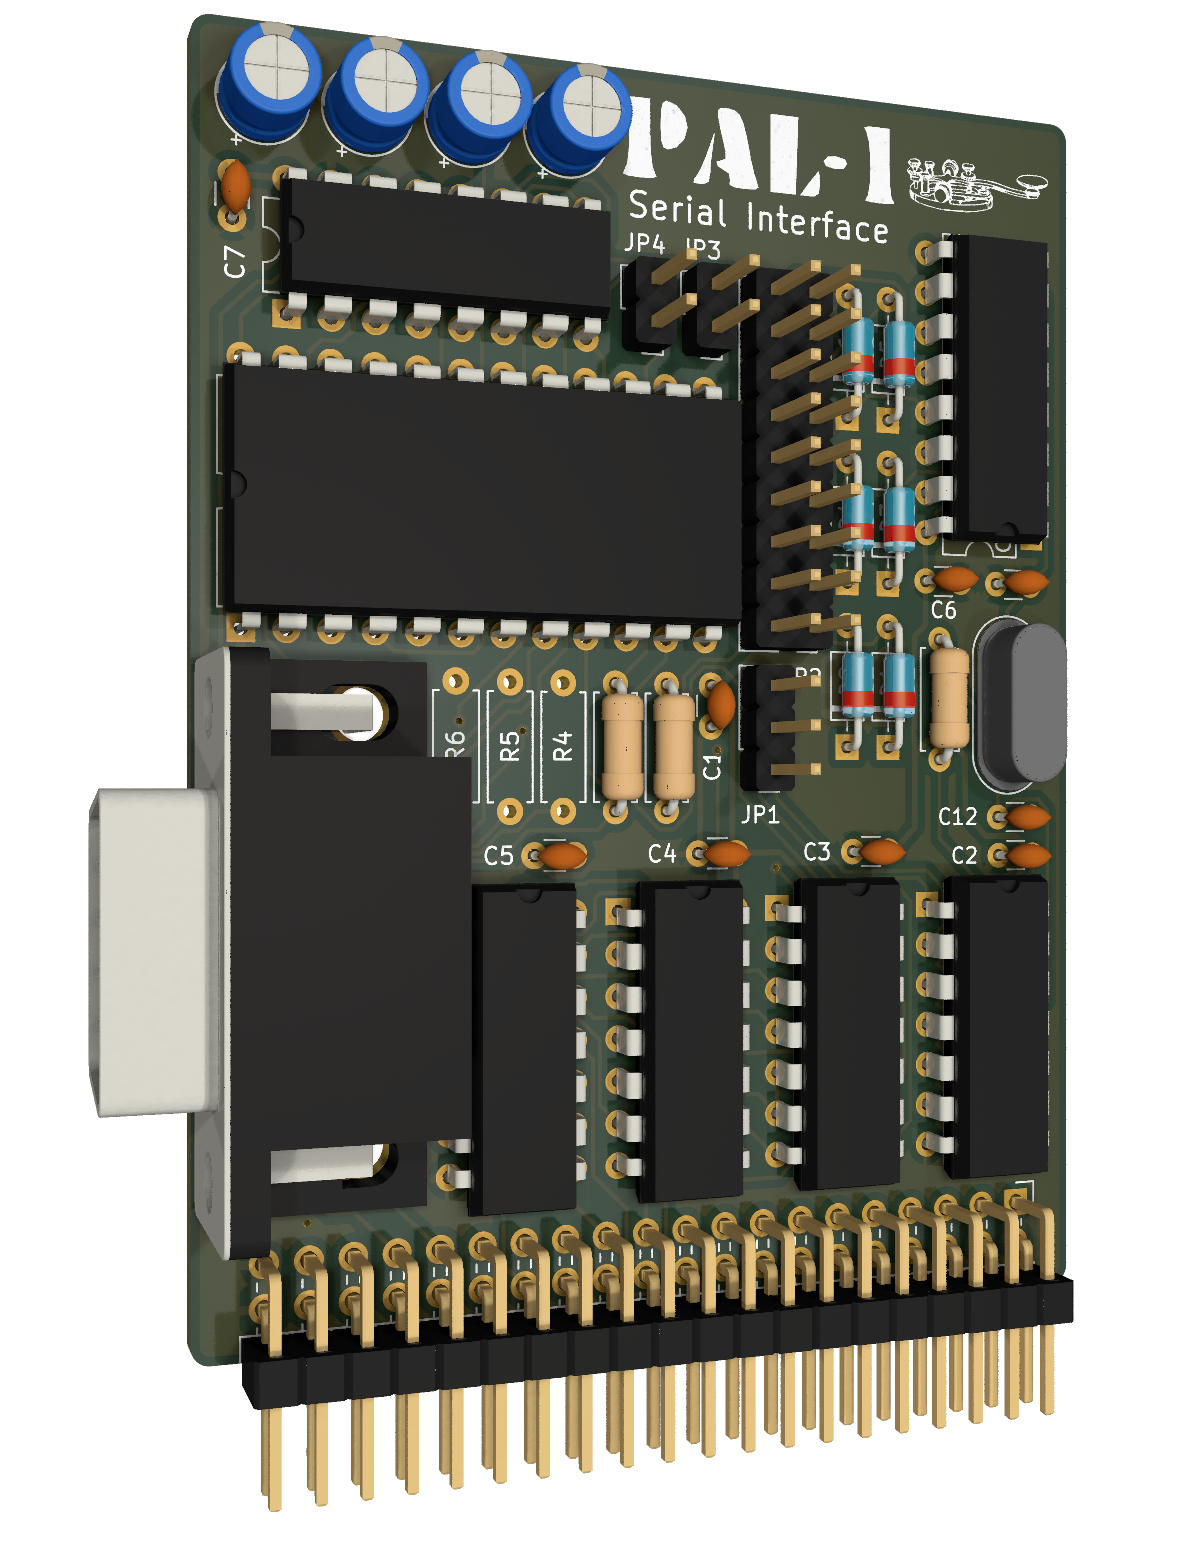
\includegraphics[scale=0.25]{figures/serial.png}
\end{figure}
\maketitle
\end{titlepage}
\clearpage
\noindent Published by \textbf{Plastic Objects Limited} \\
Woodbridge, UK

\bigskip
\noindent October 2022
\vfill
{\noindent\Large\textbf{Disclaimer}}
\vskip 6pt
Every effort has been made to ensure the accuracy of the information contained in this document. The information presented within is accurate at the time of publication. Whilst every effort is made to provide accurate information, no warranty or fitness is provided or implied, and the authors and publishers shall have neither liability nor responsibility to any person or entity with respect to any loss or damages arising from its use.

All trademarks, logos and brand names are the property of their respective owners. All company, product and service names mentioned in this document are for identification purposes only. Use of these names, trademarks and brands does not imply endorsement.

\thanks{PAL-1 and the PAL-1 logo used with kind permission of Liu Ganning.}
\clearpage
\tableofcontents
\listoffigures
\cleardoublepage
\chapter*{Introduction}
\addcontentsline{toc}{chapter}{Introduction}
The PAL-1 Serial Interface Adapter is an expansion module for the PAL\nobreakdash-1 system\cite{ganning1} based on the Motorola MC6850 Asynchronous Communications Interface Adapter (ACIA)\cite{motorola1}. The design borrows from a homebrew project in CPC Schneider International magazine\cite[pp. 88--92]{cpc1}.

The MC6850 ACIA manages data formatting and asynchronous data communications control. Data from the PAL-1 is serially transmitted and received by the ACIA's asynchronous data interface, with appropriate formatting and error checking. The functional configuration of the ACIA may be programmed during system initialisation. It includes variable word lengths, clock division ratios, and interrupt conditions giving full control over serial communications\cite[p. 11]{motorola2}.

Unlike the on-board PAL-1 serial interface, the PAL-1 Serial Interface Adapter provides hardware flow control at rates from 150 to 38400 baud. Serial connections may be made at either TTL or RS-232 levels, allowing users to connect to other devices with either a TTL-to-USB adaptor or using a 9 pin D-sub serial cable.

\mainmatter
\chapter{Getting Started}
\section*{Board assembly}
Before assembling your PAL-1 Serial Interface Adapter board check the package contents against the Bill of Materials on page \pageref{sec:bom}, and contact your distributor as soon as possible if any items are missing.

No specialist tools are required for assembling the board, though care must be taken when handling ESD sensitive components, especially the ICs. Before inserting the ICs into their sockets, check the board for dry joints and solder bridges. Also be sure to pay special attention to the orientation of the ICs, ensuring pin 1 of each IC is correctly aligned.

\awesomebox[red]{2pt}{\faHandPaper}{red}{To prevent damage to your system, \textit{always} power off your PAL-1 before installing or removing the PAL-1 Serial Interface Adapter board. Ensure that the pins are correctly aligned when inserting the board into the PAL-1 motherboard or when directly connecting it to the PAL-1 expansion port using a 40-pin IDC cable.}

\section*{Builds options}
The PAL-1 Serial Interface Adapter can be assembled with or without a MAX232 dual transmitter / dual receiver, depending on whether RS-232 or TTL level signals are preferred (see also Figure \ref{fig:alternatives}).  If only TTL level signals are required, the components listed in Table \ref{tab:notreqd} can be omitted. In this case pin-header J3 and resistors R7 to R10 should be installed to provide access to the TTL level signals (see also `\textit{TTL Pin Header}' on page \pageref{sec:ttlpins}).

\begin{figure}[!tbp]
  \begin{subfigure}[b]{0.45\textwidth}
    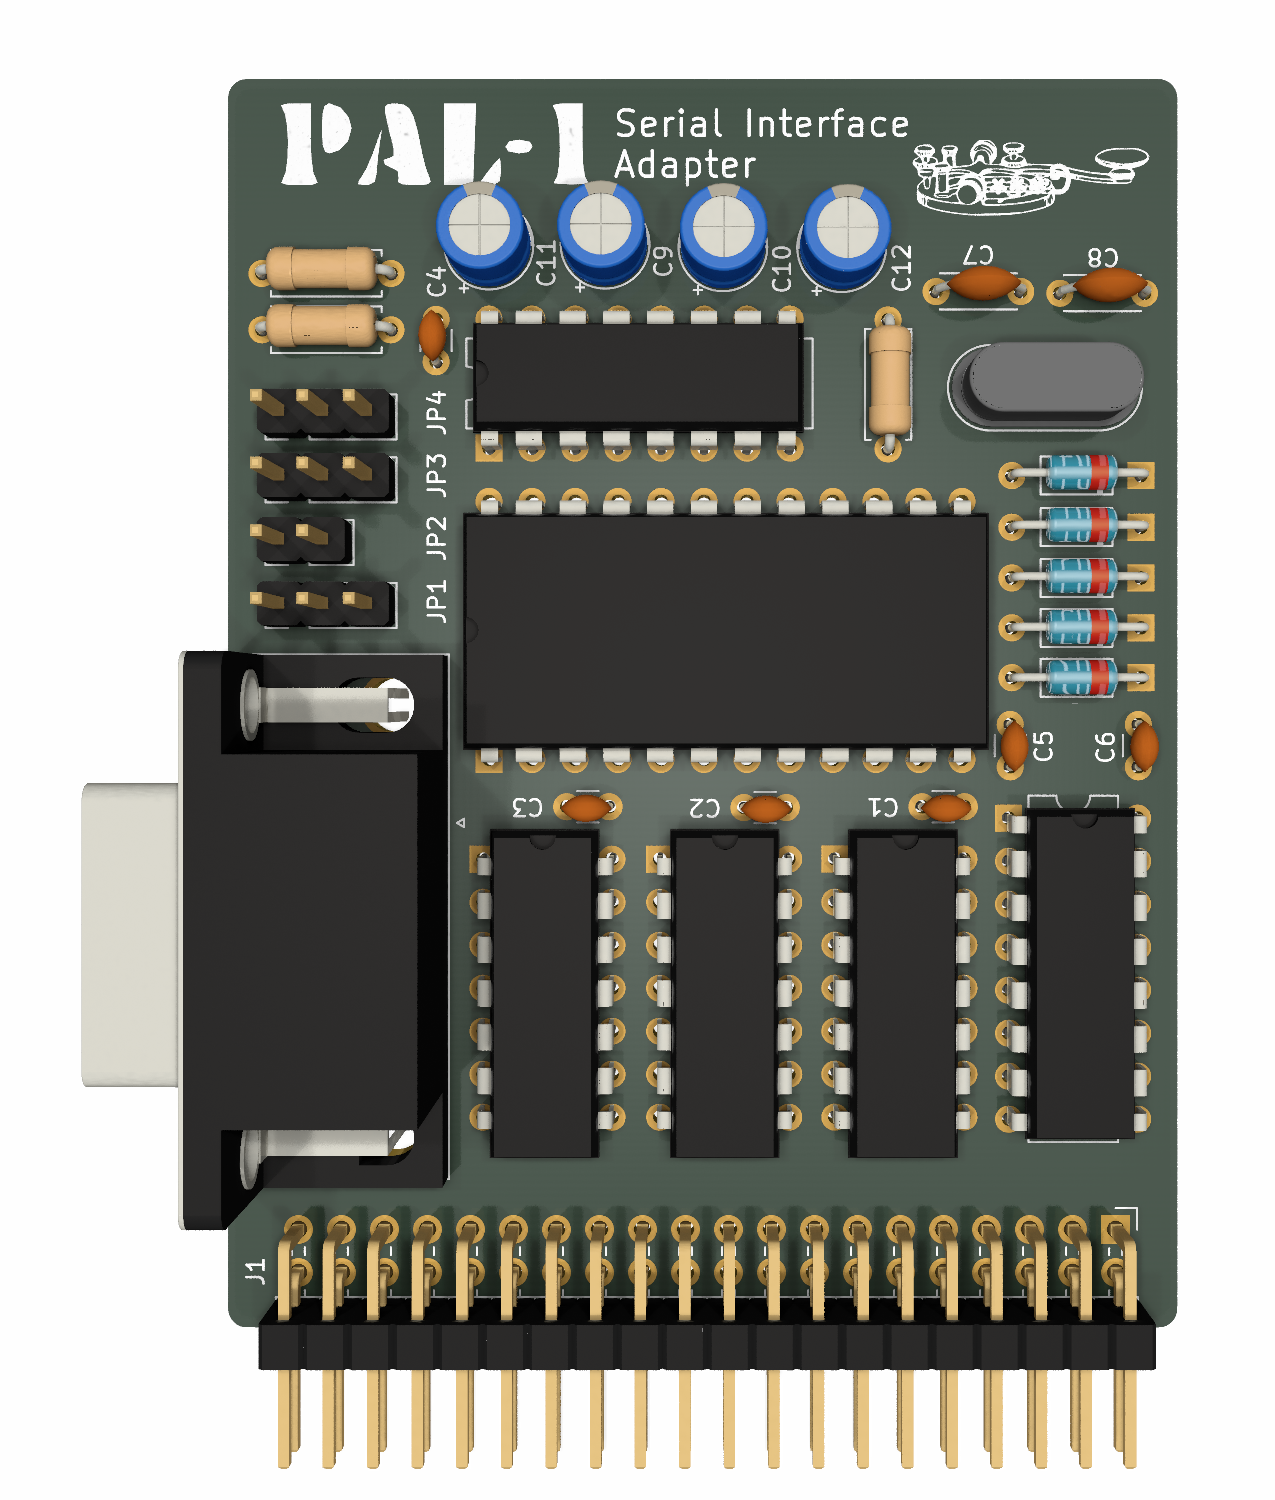
\includegraphics[width=\textwidth]{figures/serial-alt-1.png}
    \caption{With RS-232}
  \end{subfigure}
  \hfill
  \begin{subfigure}[b]{0.45\textwidth}
    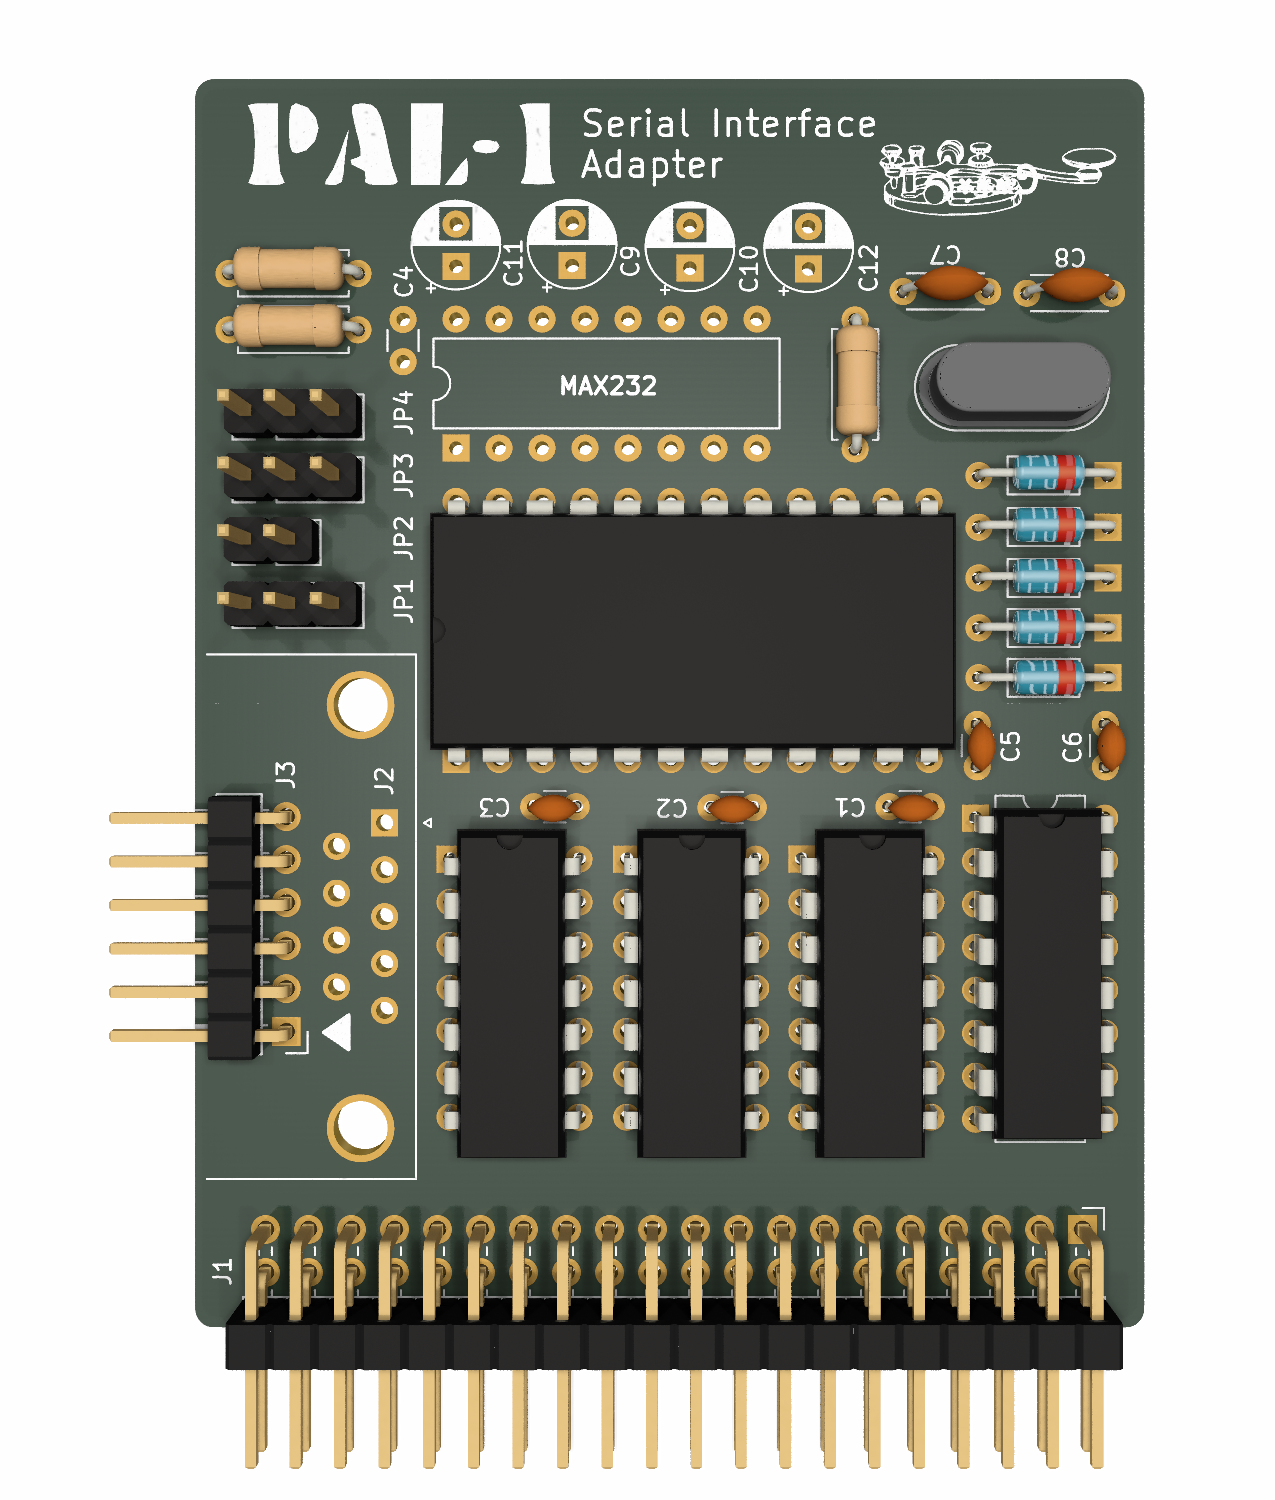
\includegraphics[width=\textwidth]{figures/serial-alt-2.png}
    \caption{TTL only}
  \end{subfigure}
  \caption{PAL-1 Serial Interface Adapter build options.}
  \label{fig:alternatives}
\end{figure}

\begin{table}[h]
\centering
\begin{tabular}{@{\extracolsep{4pt}}cl@{}}
\hline
Parts & Description \\
\cline{1-1}\cline{2-2}
C9 - C12 & 1.0uF capacitors \\
J2 & DB-9 serial connector \\
JP5 & Jumper, 2-pole, open \\
U6 & MAX232 dual transmitter / dual receiver \\
\hline
\end{tabular}
\caption[]{Components to be omitted for TTL level signals}
\label{tab:notreqd}
\end{table}

\section*{Configuration}
\label{sec:configuration}
\subsection*{Base I/O address}
The MC6850 ACIA has an 8-bit  data bus, which is memory mapped on the PAL-1 system. The base address at which it is mapped can be configured using jumper JP1, as shown in Table \ref{tab:addresses}.

The default base address (and the address used in all examples in this manual) is \$16E8. In situations where multiple serial interface adapters are installed in the same PAL-1 system, each board must have a unique base address.

\begin{table}[h]
\centering
\begin{tabular}{@{\extracolsep{4pt}}cc@{}}
\hline
JP1 pins & Address \\
\cline{1-1}\cline{2-2}
1-2 & \$16E8 ($5864_{10}$) \\
2-3 & \$16EA ($5866_{10}$) \\
\hline
\end{tabular}
\caption[]{I/O address configuration}
\label{tab:addresses}
\end{table}

\subsection*{Clock frequency}
The MC6850 ACIA uses an external clock from which data transmission rates are derived. The frequency of this clock is configured using jumpers \code{JP2} as shown in table \ref{tab:clock}. For example, to select a clock frequency of 19.2kHz, shunt pins 2, 4, 5, and 8 as shown in figure \ref{fig:clkconfig}.  \textbf{Note that only the combinations shown in this table are valid --- other settings may result in unpredictable behaviour.}

\begin{table}[h]
\centering
\begin{tabular}{@{\extracolsep{4pt}}rccccccccccc@{}}
\hline
&\multicolumn{9}{c}{JP2 pins}&\multicolumn{2}{c}{Baud rates}\\
Clock & 1 & 2 & 3 & 4 & 5 & 6 & 7 & 8 & 9 & Min & Max \\
 \cline{1-1}\cline{2-10}\cline{11-12}
9600 Hz & - & - & $\sqcap$ & - & $\sqcap$ & $\sqcap$ & - & - & $\sqcap$ & 150 & 9600 \\
19.2 kHz & - & $\sqcap$ & - & $\sqcap$ & $\sqcap$ & - & - & $\sqcap$ & - & 300 & 19,200 \\
38.4 kHz & $\sqcap$ & - & $\sqcap$ & $\sqcap$ & - & - & $\sqcap$ & - & - & 600 & 38,400 \\
\hline
\end{tabular}
\caption[]{Clock frequency configuration}
\label{tab:clock}
\end{table}

\begin{figure}[h!]
    \centering
    \scalebox{0.1}{
    \begin{tikzpicture}[font=\sffamily]
    	\draw [line width=8] (6,4) -- ++(0,9);
    	\draw [line width=8] (60,4) -- ++(0,9);
    	\draw [line width=8] (6,13)
 	\foreach \q in {1, ..., 9} { -- ++(1,1) -- ++(4,0) -- ++(1,-1) } -- ++(0,-9)
	\foreach \q in {9, ..., 1} {	-- ++(-1,-1) -- ++(-4,0) -- ++(-1,1) } -- cycle;
	\foreach \q in {9, ..., 1} {
		\draw [fill=black] (\q*6+2.25,5.5) rectangle ++(1.5,1.5);
 		\draw [fill=black] (\q*6+2.25,10) rectangle ++(1.5,1.5);
		\draw (3+\q*6, 16.5) node[scale=8,color=gray]{\q};
  	}
  	\foreach \q in {2,4,5,8} {
  		\draw [line width=6,color=black!55,line join=round] (\q*6+3.85,10) -- ++(0,1.6) -- ++(-1.7,0) -- ++(0,-6.2) -- ++(1.7,0) -- ++(0,1.6);
  		\draw [line width=1cm, color=black!80] (\q*6+1.2,4.5) rectangle ++(3.8,8);
  	}
  	\draw [line width=8] (7.5,-0.5) -- ++(3,0) -- ++(-1.5,2) -- cycle;
	\draw (64,8.5) node[scale=12, rotate=-90]{JP2};
%	\draw [-{Latex},line width=12,color=gray] (47,21) -- node[above=-1.5cm, scale=8,color=gray]{top of board} ++(20,0);
    \end{tikzpicture}
    }
    \caption{Clock set to 19.2 kHz.}
    \label{fig:clkconfig}
\end{figure}

\subsection*{Interrupts}
\label{sec:configirq}
Interrupts result from conditions in both the transmitter and receiver sections of the MC6850 ACIA. To enable interrupt handling on the PAL-1, pins \code{JP3} must be shunted. For details about ACIA interrupt processing, refer to the section on interrupts on page \pageref{sec:interrupts}.

\subsection*{Data Terminal Ready}
\label{sec:configdtr}
The MC6850 ACIA does not provide a Data Terminal Ready (DTR) signal. While normally disconnected, the DTR signal can be set to active using \code{JP4} if required by the data communications equipment (DCE). Note that the DTR signal is only available on the RS-232 connector (see also page \pageref{sec:connectors}).

\chapter{Using the Serial Interface Adapter}
The MC6850 ACIA appears on the PAL-1 as two addressable memory locations (see table \ref{tab:registers}).  Internally, the ACIA has four registers. Of these, two are read-only, the Status and Receive Data registers. The remaining two registers are write-only, the Control and Transmit Data registers.

\begin{table}[h]
\centering
\renewcommand{\arraystretch}{1.2}
\begin{threeparttable}
\begin{tabular}{@{\extracolsep{4pt}}ccl@{}}
\hline
Address\tnote{1} & Access & ACIA Register \\
\cline{1-1}\cline{2-2}\cline{3-3}
\multirow{2}{*}{\$16E8 ($5864_{10}$)} & Read & Status Register \\
 & Write & Control Register \\
\multirow{2}{*}{\$16E9 ($5865_{10}$)} & Read & Receive Data  \\
& Write & Transmit Data  \\
\hline
\end{tabular}
\begin{tablenotes}
\item[1] \footnotesize{The PAL-1 Serial Interface Adapter base address is configured using jumper \code{JP1}. See page \pageref{tab:addresses} for details.}
\end{tablenotes}
\end{threeparttable}
\caption[]{MC6850 registers}
\label{tab:registers}
\end{table}

Much of the information in this chapter is taken from the MC6850 datasheet\cite{motorola1}. Further details on the ACIA may be found in the MC6850 application note (AN-754)\cite[pp. 21--32]{motorola3}.

\subsubsection*{\textit{Master Reset}}
The \textit{master reset bits} (\code{CR0} and \code{CR1}) must be set immediately after power up to ensure the reset condition and to prepare for programming the ACIA functional configuration. After a master reset, the Control Register can be set to configure options, including clock divider ratios, word lengths, the number of stop and parity bits.

\section*{ACIA Control Register}
The MC6850 ACIA Control Register is used to configure serial communication parameters, including baud rates, word lengths, and transmission control parameters. The format of the 8-bit write only register is shown in figure \ref{fig:control}.

\begin{figure}[H]
\renewcommand{\arraystretch}{1.2}
\centering
\tcbox{
\begin{tabular}{@{\extracolsep{4pt}}cccccccc@{}}
	CR7 & CR6 & CR5 & CR4 & CR3 & CR2 & CR1 & CR0 \\
	\cline{1-1}\cline{2-3}\cline{4-6}\cline{7-8}
	IQR Enable & \multicolumn{2}{c}{Transmit Ctrl} &  \multicolumn{3}{c}{Word Select} & \multicolumn{2}{c}{Counter Divide}
\end{tabular}}
\caption{ACIA Control Register}
\label{fig:control}
\end{figure}

\subsection*{Counter Divide and Reset}
The \textit{counter divide bits} (\code{CR0} and \code{CR1}) determine the divide ratios used in both the transmitter and receiver sections of the ACIA. Additionally, these bits are used to force a master reset of the ACIA, which clears the Status Register and initialises both the receiver and transmitter. Note that after power-on or a restart these bits must be set high to reset the ACIA. After resetting the clock divide ratio may be selected. The counter select bits provide for the following clock divide ratios and corresponding baud rates:

\begin{table}[h!]
	\centering
	\begin{threeparttable}
	\begin{tabular}{@{\extracolsep{4pt}}cccccc@{}}
		\hline
		& & & \multicolumn{3}{c}{Baud rate\tnote{1}} \\
		CR1 & CR0 & Function & 9600Hz & 19.2kHz & 38.4kHz \\
		\cline{1-2}\cline{3-3}\cline{4-6}
		0 & 0 & $\div 1$ & 9600 & 19200  & 38400  \\
		0 & 1 & $\div 16$ & 600 & 1200 & 2400  \\
		1 & 0 & $\div 64$ & 150 & 300 & 600 \\
		1 & 1 & master reset  & \\
		\hline
	\end{tabular}
	\begin{tablenotes}
	\item[1] \footnotesize{Baud rates are shown for all clock frequencies.}
	\end{tablenotes}
	\end{threeparttable}
	\caption{Counter Divide / Reset bits}
\end{table}

\subsection*{Word Select}
The \textit{word select bits} (\code{CR4},\code{CR3} and \code{CR2}) are used to select word length, parity, and the number of stop bits as shown in table \ref{tab:wordselect}. Note that word length, parity select, and stop bit changes are not buffered and therefore become effective immediately.

\begin{table}[h!]
	\centering
	\begin{tabular}{@{\extracolsep{4pt}}cccccc@{}}
		\hline
		CR4 & CR3 & CR2 & Word Length & Parity & Stop bits \\
		\cline{1-3}\cline{4-6}
		0 & 0 & 0 & 7 & even & 2 \\
		0 & 0 & 1 & 7 & odd & 2 \\
		0 & 1 & 0 & 7 & even & 1 \\
		0 & 1 & 1 & 7 & odd & 1 \\
		1 & 0 & 0 & 8 & none & 2 \\
		1 & 0 & 1 & 8 & none & 1 \\
		1 & 1 & 0 & 8 & even & 1 \\
		1 & 1 & 1 & 8 & odd & 1 \\
		\hline
	\end{tabular}
	\caption{Word Select bits}
	\label{tab:wordselect}
\end{table}

\subsection*{Interrupts}
\label{sec:interrupts}
The \textit{transmitter control bits} (\code{CR5} and \code{CR6}) and the  \textit{receive interrupt enable bit} (\code{CR7}) define the circumstances under which interrupts are raised. Note that in addition to setting the relevant control register bits, pin \code{JP3} on the PAL-1 Serial Interface Adapter board must be shunted (see also page \pageref{sec:configirq}).

\subsubsection*{\textit{Transmitter Control}}
The \textit{transmitter control bits} (\code{CR5} and \code{CR6}) are used to configure the interrupt from the Transmit Data Register Empty condition, the Request to Send ($\overline{RTS}$) output, and the transmission of a Break level (space), as shown in table \ref{tab:xmit}.

\begin{table}[h!]
	\centering
	\begin{tabular}{@{\extracolsep{4pt}}cccc@{}}
		\hline
		CR5 & CR6 & $\overline{RTS}$ & Transmitter IRQ \\
		\cline{1-2}\cline{3-3}\cline{4-4}
		0 & 0 & low & disabled \\
		0 & 1 & low &  enabled \\
		1 & 0 & high & disabled \\
		1 & 1 & low & disabled and break \\
		\hline
	\end{tabular}
	\caption{Transmitter Control bits}
	\label{tab:xmit}
\end{table}

\subsubsection*{\textit{Receiver Interrupt Enable}}
Setting the \textit{receiver interrupt enable bit} (\code{CR7}) will enable interrupts for the following conditions: Receive Data Register fill, Overrun, or a low-to-high transition on the Data Carrier Detect ($\overline{DCD}$) signal line.

\section*{ACIA Status Register}

The status of the MC7850 ACIA may be read from the ACIA Status Register. The information stored in this register indicates the status of the Transmit Data Register, the Receive Data Register and error logic, and the peripheral status inputs of the ACIA.

\begin{figure}[H]
\renewcommand{\arraystretch}{1.2}
\centering
\tcbox{
\begin{tabular}{@{\extracolsep{4pt}}cccccccc@{}}
	SR7 & SR6 & SR5 & SR4 & SR3 & SR2 & SR1 & SR0 \\
	\cline{1-1}\cline{2-2}\cline{3-3}\cline{4-4}\cline{5-5}\cline{6-6}\cline{7-7}\cline{8-8}
	\small{$\overline{IRQ}$} & \small{PE} & \small{OVRN} & \small{FE} & \small{$\overline{CTS}$} &  \small{$\overline{DCD}$} & \small{TDRE} & \small{RDRF}
\end{tabular}}
\caption{ACIA Status Register}
\end{figure}.

\subsection*{Receive Data Register Full (RDRF)}
The \textit{receive data register full bit} (\code{SR0}) indicates that received data has been transferred to the receive data register. The \textit{receive data register full bit} is cleared when the Receive Data Register is read or by a master reset. When the \textit{receive data register full bit} is not set the data in the Receive Data Register is not current.

\subsection*{Transmit Data Register Empty (TDRE)}
The \textit{transmit data register empty bit} (\code{SR1}) is set when the contents of the Transmit Data Register have been transferred, indicating that new data may be entered. When the \textit{transmit data register empty} is not set, the transmission of the character currently in the Transmit Data Register has not yet begun.

\subsection*{Data Carrier Detect ($\overline{DCD}$)}
The \textit{data carrier detect bit} (\code{SR2}) would normally indicate the modem carrier status. However, as the $\overline{DCD}$ pin of the MC6850 is permanently connected to ground on the PAL-1 Serial Interface Adapter,  the \textit{data carrier detect bit} will never be set.

\subsection*{Clear-to-Send ($\overline{CTS}$)}
The \textit{clear to send bit} (\code{SR3}) indicates the Clear-to-Send input from the modem. A low $\overline{CTS}$ indicates that there is a Clear-to-Send from the modem. In the high state, the Transmit Data Register Empty bit is inhibited and the Clear-to-Send status bit will be high. Master reset does not affect  the Clear-to-Send status bit.

\subsection*{Framing Error (FE)}
The \textit{framing error bit} (\code{SR4}) indicates that the received character is improperly framed by a start and stop bit. Framing errors are detected by the absence of the first stop bit. This error indicates a synchronisation error, a faulty transmission, or a break condition. The framing error bit is set or reset during the receive data transfer time. Therefore, this error indicator is present throughout the time that the associated character is available.

\subsection*{Receive Overrun (OVRN)}
A receive overrun error indicates that one or more characters in the data stream were lost. This happens when a character or number of characters were received, but not read from the Receive Data Register prior to subsequent characters being received. The \textit{receive overrun bit} (\code{SR5}) is reset after reading data from the Receive Data Register, or by a master reset.

\subsection*{Parity Error (PE)}
The \textit{parity error bit} (\code{SR6}) is set when the number of highs (ones) in the character does not agree with the preset odd or even parity. If no parity is selected then both the transmitter parity generator output and receiver parity check results are inhibited.

\subsection*{Interrupt Request ($\overline{IQR}$)}
The \textit{interrupt request bit} (\code{SR7}) indicates that an interrupt has occurred. This status bit may be set by any enabled interrupt condition. It is cleared when the Receive Data Register is read, or when a character is written to the Transmit Data Register.

\documentclass[a4paper,11pt]{article}
\usepackage[lmargin=142pt,rmargin=95pt,tmargin=127pt,bmargin=123pt]{geometry}
\usepackage{xcolor}
\usepackage{tikz}
\usetikzlibrary{shapes.arrows,arrows.meta}
\usepackage{caption}
\newcommand{\chapter}{\section*}
\captionsetup[table]{labelformat=empty}
\begin{document}
\chapter{PAL-1 Serial Interface Adapter Block Diagram}
\label{sec:blockdiagram}
\begin{figure}[h!]
  \begin{center}
  \scalebox{0.2}{
    \begin{tikzpicture}[font=\sffamily,rotate=90,transform shape]

    	\draw (20, 10) rectangle ++(10,10) node[pos=.5,scale=4,text width=2cm,align=center] {Receive Data Register};	
    	\draw (20, 23) rectangle ++(10,10) node[pos=.5,scale=4,text width=2cm,align=center] {Control Register};	
    	\draw (20, 37) rectangle ++(10,10) node[pos=.5,scale=4,text width=2cm,align=center] {Status Register};
    	\draw (20, 52) rectangle ++(10,10) node[pos=.5,scale=4,text width=2cm,align=center] {Transmit Data Register};		
	\draw (35,11) rectangle ++(12,8) node[pos=.5,scale=4,text width=2cm,align=center] {Receive Shift  Register};
	\draw (35,53) rectangle ++(12,8) node[pos=.5,scale=4,text width=2cm,align=center] {Transmit Shift  Register};
	\draw(35,3) rectangle ++(7,5) node[pos=0.5,scale=4,text width=1.5cm,align=center] {Clock Gen};
	\draw(45,3) rectangle ++(7,5) node[pos=0.5,scale=4,text width=1.5cm,align=center] {Sync Logic};
	\draw(35,64) rectangle ++(7,5) node[pos=0.5,scale=4,text width=1.5cm,align=center] {Clock Gen};
	\draw(45,64) rectangle ++(7,5) node[pos=0.5,scale=4,text width=1.5cm,align=center] {Parity Gen};
	\draw(36,22) rectangle ++(10,5) node[pos=.5,scale=4,text width=2cm,align=center] {Receive Control};
	\draw(36,45) rectangle ++(10,5) node[pos=.5,scale=4,text width=2cm,align=center] {Transmit Control};
	\draw(52,22) rectangle ++(7,5) node[pos=0.5,scale=4,text width=1.5cm,align=center] {Parity Check};
	\draw(45.5,35) rectangle ++(10,5) node[pos=0.5,scale=4,text width=1.5cm,align=center] {Interrupt Logic};
	\draw(2,23) rectangle ++(8,26) node[pos=0.5,scale=4,text width=1.5cm,align=center] {Data Bus Buffers};
	\draw(2,52) rectangle ++(8,10) node[pos=0.5,scale=4,text width=2.5cm,align=center] {Chip Select \\and\\Read/Write Control};
	\draw(-8,57) rectangle ++(7,5) node[pos=0.5,scale=4,text width=1.5cm,align=center] {Address Decoder};
	\draw(-8,65) rectangle ++(7,5) node[pos=0.5,scale=4,text width=1.5cm,align=center] {Clock Source};
	\draw(-21,30) rectangle ++(8,32) node[pos=0.5,scale=4,text width=1.5cm,align=center] {PAL-1 MOS 6502 CPU};
	\draw[dash pattern=on 10pt off 10pt](61,12) rectangle ++(6.25,50)
			node[pos=0.5,scale=4,text width=1.5cm,align=center] {RS-232 Drivers/ Receivers};
	
	\draw[-{Latex[scale=5]}](62,15) -- ++(-15,0);
	\draw[arrows={Latex[scale=5]-Latex[scale=5]}](52,5.5) -- ++(3.5,0) -- ++(0,16.5);
	\draw[arrows={Latex[scale=5]-Latex[scale=5]}](50.5,40) -- ++(0,2) -- ++(-20.5,0);
	\draw[arrows={Latex[scale=5]-Latex[scale=5]}](49.50,64) -- ++(0,-4.5) -- ++(-2.5,0);
	\draw[-{Latex[scale=5]}](38.5,8) -- ++(0,3);
	\draw[-{Latex[scale=5]}](41,50) -- ++(0,3);
	\draw[-{Latex[scale=5]}](45,5.5) -- ++(-3,0);
	\draw[-{Latex[scale=5]}](41,22) -- ++(0,-3);
	\draw[-{Latex[scale=5]}](38.5,64) -- ++(0,-3);
	\draw[-{Latex[scale=5]}](6,52) -- ++(0,-3);
	\draw[-{Latex[scale=5]}](-1,59.5) -- ++(3,0);
	\draw[-{Latex[scale=5]}](52,24.5) -- ++(-6,0);
	\draw[-{Latex[scale=5]}](30,24.5) -- ++(6,0);
	\draw[-{Latex[scale=5]}](-13,54) -- ++(15,0);
	\draw[-{Latex[scale=5]}](41,27) -- ++(0,12) -- ++(-11,0);
	\draw[-{Latex[scale=5]}](50.5,46.5) -- ++(0,-3) -- ++(-20.5,0);		
	\draw(22,33) -- ++(0,2) -- ++(-3.5,0) -- ++(0,6.75);
	\draw[-{Latex[scale=5]}](18.5,43.25) -- ++(0,5.25) -- ++(17.5,0);
	\draw[-{Latex[scale=5]}](-1,67.5) -- ++(36,0);
	\draw(47,57) -- ++(14.75,0);
	\draw(13,67.5) -- ++(0,-20);
	\draw(13,46) -- ++(0,-2.75);				
	\draw(13,41.75) -- ++(0,-11.5);	
	\draw(13,28.75) -- ++(0,-2.75);		
	\draw[-{Latex[scale=5]}](13,24.5) -- ++(0,-19) -- ++(22,0);
	
	\draw[fill=black] (55.5,15) circle (2mm);
	\draw[fill=black] (50.5,46.5) circle (2mm);
	\draw[fill=black] (13,67.5) circle (2mm);
		
	\draw[{Circle[open,scale=6,line width=2]}-](30,31.5) -- ++(31.75,0);
	\draw[arrows={Circle[open,scale=6,line width=2]-Latex[scale=5]}](50.5,35) -- ++(0,-26) -- 
			++(-67.5,0) -- ++(0,21);
	\draw[{Circle[open,scale=6,line width=2]}-](46,46.5) -- ++(16,0);
	
	\draw (35,15) node [draw,single arrow, minimum height=5cm, minimum width=4cm,
	                             anchor=west,line width=1,rotate=180] {};
	\draw (30,57) node [draw,single arrow, minimum height=5cm, minimum width=4cm,
	                             anchor=west,line width=1] {};
	\draw (10,29.5) node [draw,single arrow, minimum height=10cm, minimum width=4cm,
	                             anchor=west,line width=1] {};
	\draw (20,42.5) node [draw,single arrow, minimum height=10cm, minimum width=4cm,
	                             anchor=west,line width=1,rotate=180] {};
	\draw (-13,59.5) node [draw,single arrow, minimum height=5cm, minimum width=4cm,
	                             anchor=west,line width=1] {};
	                             
	\draw[line width=1](10,46) -- ++(5.5,0) -- ++(0,10.25) -- ++(2.5,0) -- ++(0,-1.25) -- ++(2,2) -- 
			++(-2,2) -- ++(0,-1.25) -- ++(-4,0) -- ++(0,-10.25) -- ++(-4,0) -- cycle;
	\draw[line width=1](20,14.25) -- ++(-5.5,0) -- ++(0,10.25) -- ++(-2.5,0) -- ++(0,-1.25) -- ++(-2,2) --
			++(2,2) -- ++(0,-1.25) -- ++(4,0) -- ++(0,-10.25) -- ++(4,0) -- cycle;
	\draw[line width=1](-13,39.5) -- ++(2,2) -- ++(0,-1.25) -- ++(11,0) -- ++(0,1.25) -- ++(2,-2) --
			++(-2,-2) -- ++(0,1.25) -- ++(-11,0) -- ++(0,-1.25) -- cycle;
			
	\draw[line width=1](61.75,46.5) -- ++(4,2) -- ++(0,-4) -- cycle;
	\draw[{Circle[open,scale=6,line width=2]}-](65.75,46.5) -- ++(4,0);
	\draw[line width=1](61.75,15) -- ++(4,2) -- ++(0,-4) -- cycle;
	\draw[{Circle[open,scale=6,line width=2]}-](65.75,15) -- ++(4,0);
	
	\draw[line width=1](61.75,59) -- ++(4,-2) -- ++(-4,-2) -- cycle;
	\draw[arrows={Circle[open,scale=6,line width=2]-Latex[scale=5]}](65.75,57) -- ++(4,0);
	\draw[line width=1](61.75,33.5) -- ++(4,-2) -- ++(-4,-2) -- cycle;
	\draw[arrows={Circle[open,scale=6,line width=2]-Latex[scale=5]}](65.75,31.5) -- ++(4,0);

	\node[anchor=west,scale=4] at (70,57) {TxD};
	\node[anchor=west,scale=4] at (70,46.5) {CTS};
	\node[anchor=west,scale=4] at (70,31.5) {RTS};
	\node[anchor=west,scale=4] at (70,15) {RxD};
	\node[anchor=north,scale=4] at (64,62) {optional};
    \end{tikzpicture}
    }
    \caption{PAL-1 Serial Interface Adapter block diagram.}
  \end{center}
\end{figure}

\end{document} 





\clearpage
\section*{Hardware flow control}
Devices process data at different rates. When transferring data from a faster device to a slower one, data may be lost unless the slower device is able to control the flow of data. Such flow control may be implemented using different methods. When using \textit{software flow control}, special characters are sent via the data lines to pause and resume the flow of data. Alternatively, \textit{hardware flow control} signals the pausing and resumption of data flows using additional wire connections between the communicating devices. Hardware flow control may be implemented in two different ways, as discussed below.

\subsubsection*{Hardware flow control}
To implement hardware flow control, RTS (\textit{Request to Send}) and CTS (\textit{Clear to Send}) need to be cross-coupled (as shown in figure \ref{fig:flowctl}). Each device uses RTS to indicate that it is ready to accept data. Before sending any data a device needs to check CTS to ensure that the remote device is in a state to receive data.

\vspace{1em}
\begin{figure}[H]
	\begin{center}
		\def\radius{6mm}
		\scalebox{0.4}{
			\begin{tikzpicture}[font=\sffamily]
				\draw[line width=1, fill=black!60] (0,0) rectangle ++(10,10);
				\draw[line width=1, fill=black!60] (20,0) rectangle ++(10,10);
				\draw (5,9) node[scale=2.75,black!5]{DEVICE A};
				\draw (25,9) node[scale=2.75,black!5]{DEVICE B};

				\foreach \p [count=\q from 0] in {{GND},{RTS},{CTS},{RX},{TX}}{
					\node (rect) at (10, 1+\q*1.7) [draw,thick,minimum width=1cm,minimum height=1cm,fill=white,label={[white,scale=2] left:\p}] (l-\p){};
					\node (rect) at (20, 1+\q*1.7) [draw,thick,minimum width=1cm,minimum height=1cm,fill=white,label={[white,scale=2] right:\p}] (r-\p){};
				}

				\draw [-{Latex[length=1cm, round]},line width=1mm,name path=line 1] (r-TX) -- (l-RX);
				\path[name path=line 2] (l-TX) -- (r-RX);
				\path [name intersections={of = line 1 and line 2, name=i}];
				\coordinate (S) at (i-1);
				\path[name path=c1] (S) circle(\radius);
				\path [name intersections={of = c1 and line 2, name=i}];
				\coordinate (I1)  at (i-2);
				\coordinate (I2)  at (i-1);
				\draw[line width=1mm] (l-TX) -- (I2);
				\draw[-{Latex[length=1cm, round]},line width=1mm] (I1) -- (r-RX);
				\tkzDrawArc[line width=1mm](S,I1)(I2);

				\draw [-{Latex[length=1cm, round]},line width=1mm,name path=line 3] (r-CTS) -- (l-RTS);
				\path[name path=line 4] (l-CTS) -- (r-RTS);
				\path [name intersections={of = line 3 and line 4, name=i}];
				\coordinate (T) at (i-1);
				\path[name path=c2] (T) circle(\radius);
				\path [name intersections={of = c2 and line 4, name=i}];
				\coordinate (I3)  at (i-1);
				\coordinate (I4)  at (i-2);
				\draw[line width=1mm] (l-CTS) -- (I3);
				\draw[-{Latex[length=1cm, round]},line width=1mm] (I4) -- (r-RTS);
				\tkzDrawArc[line width=1mm](T,I4)(I3);

				\draw [line width=1mm] (l-GND) -- (r-GND);

			\end{tikzpicture}
		}
		\captionof{figure}{Hardware flow control.}
		\label{fig:flowctl}
	\end{center}
\end{figure}

A device will keep its RTS line asserted while it is ready to accept data. To ensure no data is lost, a device needs to negate RTS well before its receive buffer is full. No data should be sent to a device until RTS is asserted.

This implementation allows for bi-directional flow control; either device may request that data transmission is halted or resumed.

\subsubsection*{Legacy hardware flow control}
In legacy systems hardware flow control is uni-directional, with the \textit{Data Terminal Equipment} (DTE) managing the rate of flow to and from the \textit{Data Communication Equipment} (DCE). In such systems the RTS (\textit{Request to Send}) and CTS (\textit{Clear to Send}) connections are wired straight through, rather than being cross-coupled (see figure \ref{fig:legacyctl}).

\vspace{1em}
\def\radius{6mm}
\begin{figure}[H]
	\begin{center}
		\scalebox{0.4}{
			\begin{tikzpicture}[font=\sffamily]
				\draw[line width=1, fill=black!60] (0,0) rectangle ++(10,10);
				\draw[line width=1, fill=black!60] (20,0) rectangle ++(10,10);
				\draw (5,9) node[scale=2.75,black!5]{DTE};
				\draw (25,9) node[scale=2.75,black!5]{DCE};

				\foreach \p [count=\q from 0] in {{GND},{RTS},{CTS},{RX},{TX}}{
					\node (rect) at (10, 1+\q*1.7) [draw,thick,minimum width=1cm,minimum height=1cm,fill=white,label={[white,scale=2] left:\p}] (l-\p){};
					\node (rect) at (20, 1+\q*1.7) [draw,thick,minimum width=1cm,minimum height=1cm,fill=white,label={[white,scale=2] right:\p}] (r-\p){};
				}

				\draw [-{Latex[length=1cm, round]},line width=1mm,name path=line 1] (r-TX) -- (l-RX);
				\path[name path=line 2] (l-TX) -- (r-RX);
				\path [name intersections={of = line 1 and line 2, name=i}];
				\coordinate (S) at (i-1);
				\path[name path=c1] (S) circle(\radius);
				\path [name intersections={of = c1 and line 2, name=i}];
				\coordinate (I1)  at (i-2);
				\coordinate (I2)  at (i-1);
				\draw[line width=1mm] (l-TX) -- (I2);
				\draw[-{Latex[length=1cm, round]},line width=1mm] (I1) -- (r-RX);
				\tkzDrawArc[line width=1mm](S,I1)(I2);

				\draw [line width=1mm,{Latex[length=1cm, round]}-] (l-CTS) -- (r-CTS);
				\draw [line width=1mm,-{Latex[length=1cm, round]}] (l-RTS) -- (r-RTS);
				\draw [line width=1mm] (l-GND) -- (r-GND);

			\end{tikzpicture}
		}
		\caption{Legacy hardware flow control.}
		\label{fig:legacyctl}
	\end{center}
\end{figure}

When it wants to transmit data, the DTE asserts RTS. If the DCE is in a state to accept data, it responds by asserting CTS. Transmission continues until the DCE negates CTS. When the DTE has completed transmitting data it negates RTS.


\chapter{Sample Code}

Programming the PAL-1 Serial Interface Adapter simply requires the ability to write to and read from the mapped I/O address. Many programming languages provide statements to achieve this, including the \code{POKE} and \code{PEEK} statements in BASIC, and \code{C!} and \code{C@} in Forth.

Note that all examples included below use the default base address (ie. \$16E8, $5864_{10}$).  Further examples may be found on Github at \url{https://github.com/dimitrit/pal1serial}.

\subsection*{BASIC}

The following example was taken from the `\textit{Do-It-Yourself RS-232 Interface}' article in the 1986 Special Edition, Issue 3 of CPC Schneider International magazine\cite[pp. 88--92]{cpc1}. Because the MC6850 ACIA is memory mapped on the PAL-1 all \code{OUT} statements have been replaced with \code{POKE} statements, and \code{IN} with \code{PEEK}. Note that this example requires loopback connections from \code{TXD} to \code{RXD}, and from \code{RTS} to \code{CTS}.

\lstinputlisting[basicstyle=\footnotesize\ttfamily,caption={RS-232 test program},captionpos=b,
	language={[Visual]Basic},label={lst:sample1},frame=single]{../examples/basic/TEST.BAS}

\subsection*{6502 assembly language}

The assembly language example shown below implements a simple terminal application. Characters read from the TTY device connected to the PAL-1 are sent to the Serial Adapter, and vice versa. As this example uses interrupts to process received characters, \code{JP3} on the Serial Adapter Interface must be closed (see also page \pageref{sec:configirq}).

\lstinputlisting[basicstyle=\footnotesize\ttfamily,caption={MiniTerm program listing},
	captionpos=b,language={[Motorola68k]Assembler},
	label={lst:sample2},frame=single]{../examples/asm/miniterm.a65}

\appendix

\chapter{Connector Pin Outs}
\label{sec:connectors}
\subsection*{RS-232 D-Sub Connector}
The pin-out of the RS-232 D-Sub 9-pin male connector (J2) follows the standard convention for Data Terminal Equipment (DTE), as shown in Figure \ref{fig:dsub9}.

\begin{figure}[h!]
  \begin{center}
  \scalebox{0.2}{
    \begin{tikzpicture}[font=\sffamily]
    	\draw[rounded corners=2cm,line width=6mm] (0, 0) rectangle (25,10) {};

    	\draw[line width=4mm] (3,5) circle (1.4cm);
    	\draw[line width=4mm] (22,5) circle (1.4cm);

    	\draw[line width=1mm] (7,8) -- (18,8);
    	\draw[line width=1mm] (8,2) -- (17,2);
    	\draw[line width=1mm] (6,7) -- (7,3);
    	\draw[line width=1mm] (19,7) -- (18,3);
    	\draw[line width=1mm] (6,7) to[out=102,in=180,distance=22] (7,8);
    	\draw[line width=1mm] (7,3) to[out=-78,in=180,distance=22] (8,2);
    	\draw[line width=1mm] (17,2) to[out=0,in=-102,distance=22] (18,3);
    	\draw[line width=1mm] (19,7) to[out=78,in=0,distance=22] (18,8);

    	\draw[line width=1mm] (7,8.5) -- (18,8.5);
    	\draw[line width=1mm] (8,1.5) -- (17,1.5);
    	\draw[line width=1mm] (5.5,7) -- (6.5,3);
    	\draw[line width=1mm] (19.5,7) -- (18.5,3);
    	\draw[line width=1mm] (5.5,7) to[out=102,in=180,distance=30] (7,8.5);
    	\draw[line width=1mm] (6.5,3) to[out=-78,in=180,distance=30] (8,1.5);
    	\draw[line width=1mm] (17,1.5) to[out=0,in=-102,distance=30] (18.5,3);
    	\draw[line width=1mm] (19.5,7) to[out=78,in=0,distance=30] (18,8.5);

	\foreach \p\k [count=\q from 0] in {{}/{},{RXD}/{RTS},{TXD}/{CTS},{DTR}/{},{GND}/{}} {
		\draw[line width=1mm] (8.4+\q*2,6.2) circle (4mm);
		\ifthenelse{\q<4}{\draw[line width=1mm] (9.4+\q*2,3.8) circle (4mm);	}{}
		\foreach \x in \p {
			\draw[line width=1mm,gray] (8.4+\q*2,6.6) -- ++(0,6);
			\draw (8.4+\q*2,14.5) node[rotate=-90,scale=4]{\p};
		}{}
		\foreach \x in \k {
			\draw[line width=1mm,gray] (9.4+\q*2,3.4) -- ++(0,-6);
			\draw (9.4+\q*2,-4.8) node[rotate=-90,scale=4,text width=1cm]{\k};
		}
		\draw (7.4,6.6) node[scale=3,gray]{1};
		\draw (17.45,6.6) node[scale=3,gray]{5};
		\draw (8.4,3.4) node[scale=3,gray]{6};
		\draw (16.45,3.4) node[scale=3,gray]{9};
	}
    \end{tikzpicture}
    }
    \caption{D-Sub 9-Pin Male Connector}
    \label{fig:dsub9}
  \end{center}
\end{figure}

\begin{table}[h!]
	\centering
	\begin{threeparttable}
	\begin{tabular}{@{\extracolsep{4pt}}cll@{}}
		\hline
		Pin & Signal & Description \\
		\cline{1-1}\cline{2-2}\cline{3-3}
		1 & {\color{gray}NC} & {\color{gray}Not Connected} \\
		2 & RXD & Receive Data  \\
		3 & TXD & Transmit Data \\
		4 & DTR & Data Terminal Ready\tnote{1}  \\
		5 & GND & Ground \\
		6 & {\color{gray}NC} & {\color{gray}Not Connected} \\
		7 & RTS & Request to Send  \\
		8 & CTS\# & Clear to Send  \\
		9 & {\color{gray}NC} & {\color{gray}Not Connected}  \\
		\hline
	\end{tabular}
	\begin{tablenotes}
	\item[1] \footnotesize{DTR is set using \code{JP5} (see page \pageref{sec:configdtr}).}
	\end{tablenotes}
	\end{threeparttable}
	\caption{D-Sub 9-Pin Male Connector}
	\label{tab:rs232pins}
\end{table}

\clearpage
\subsection*{TTL Pin Header}
\label{sec:ttlpins}
The PAL-1 Serial Adapter TTL pin header (J3) allows 6-way FTDI based USB to TTL converters to be directly connected\cite[pp. 11--12]{ftdi1}.  \textbf{Be sure to check the USB to TTL converter voltage levels and signals before connecting as incorrect voltage and/or incompatible signals may result in damage to the PAL-1 Serial Adapter.}

\documentclass[a4paper,11pt]{article}
\usepackage{xcolor}
\usepackage{tikz}
\usetikzlibrary{shapes.arrows,arrows.meta}
\begin{document}
\begin{figure}[h!]
    \scalebox{0.08}{
    \begin{tikzpicture}[font=\sffamily]
 	\foreach \p [count=\q from 0] in {{GND},{RTS\char"0023},{NC},{RXD},{TXD},{CTS\char"0023}}{
  		\draw[line width=1, fill=gray!80] (4.5, 0+\q*6.5) rectangle ++(19,2) {};
		\draw (-1, 1+\q*6.5) node[scale=8,text width=1cm,align=right]{\p};   		
   	}   	
   	\draw[line width=1mm, fill=black] (16, -2) rectangle ++(5,39) {};
  	\foreach \i in {0,...,5} {
  	   	\draw[line width=1, fill=black!80] (16.5,-1+\i*6.5) rectangle ++(4,4) {};
 	   	\draw[line width=1, fill=black!90] (21,-0.5+\i*6.5) rectangle ++(0.3,3);
  	}
	\draw (23.5,36.5) node[scale=7,black!90]{6};
	\draw (23.5,-2) node[scale=7,black!90]{1};
	
	\draw[line width=1,fill=black](-60,-2) rectangle ++(36,40){};
	\draw[line width=1,fill=gray](-24,-2) -- ++(2,2) -- ++(0,35) -- ++(-2,3) -- cycle;
	
	\draw[fill=black] (-85,17.5) ellipse (1cm and 4cm);
	\draw[fill=black] (-120,20) ellipse (1cm and 4cm);
	\draw[line width=8cm] (-85,17.5) to [out=180,in=0] (-120,20);
	%\draw (-121,12) node[scale=10] (arrow) {$\leftarrow$};
	%\node[scale=10, below of=arrow, node distance=1em] {USB};
	
 	\foreach \p/\c [count=\q from 0] in {{RTS\char"0023}/{green},{RXD}/{yellow},{TXD}/{orange},{+5V}/{red},{CTS\char"0023}/{brown},{GND}/{black}} {
  		\draw[fill=black](-23.5,-1+6.5*\q) -- (-23.5,4+6.5*\q) -- (-22.5,5+6*\q) -- (-22.5,0.2+6*\q);
		\draw (-43, 34-\q*6.5) node[scale=8,text width=1cm,align=center,text=gray!20]{\p};   	
		\draw[line width=28,line cap=round,color=\c] (-60,33-\q*6) to [out=180,in=0] (-85,20-\q);	
   	}   	
	\draw[fill=gray!30] (-27,0) -- ++(0,3) -- ++(2,-1.5) -- cycle;
	\draw[line width=1,fill=black](-60,-2) rectangle ++(2,40){};
	
    \end{tikzpicture}
    }
    \caption{TTL Pin Header}
    \label{fig:ttlpins}
\end{figure}
\end{document} 





\begin{table}[h!]
	\centering
	\begin{tabular}{@{\extracolsep{4pt}}cllcl@{}}
		\hline
		Pin & Signal & Description & TTL-232R-5V & Signal\\
		\cline{1-3}\cline{4-5}
		1 & GND & Ground & Black & GND \\
		2 & RTS\# & Request to Send & Brown & CTS\# \\
		3 & {\color{gray}NC} & {\color{gray}Not Connected} & Red & 5V \\
		4 & RXD & Receive Data & Orange & TXD \\
		5 & TXD & Transmit Data & Yellow & RXD \\
		6 & CTS\# & Clear to Send & Green & RTS\# \\
		\hline
	\end{tabular}
	\caption{TTL Pin Header \& FTDI USB Adapter Connections}
	\label{tab:ttlpins}
\end{table}

\documentclass[a4paper,11pt]{article}
%\usepackage[lmargin=142pt,rmargin=95pt,tmargin=127pt,bmargin=123pt]{geometry}
\usepackage{rotating}
\newcommand{\chapter}{\section*}
\begin{document}
\chapter{Schematic Diagram}
\begin{figure}[p]
    \vspace*{-2cm}
    \makebox[\linewidth]{
        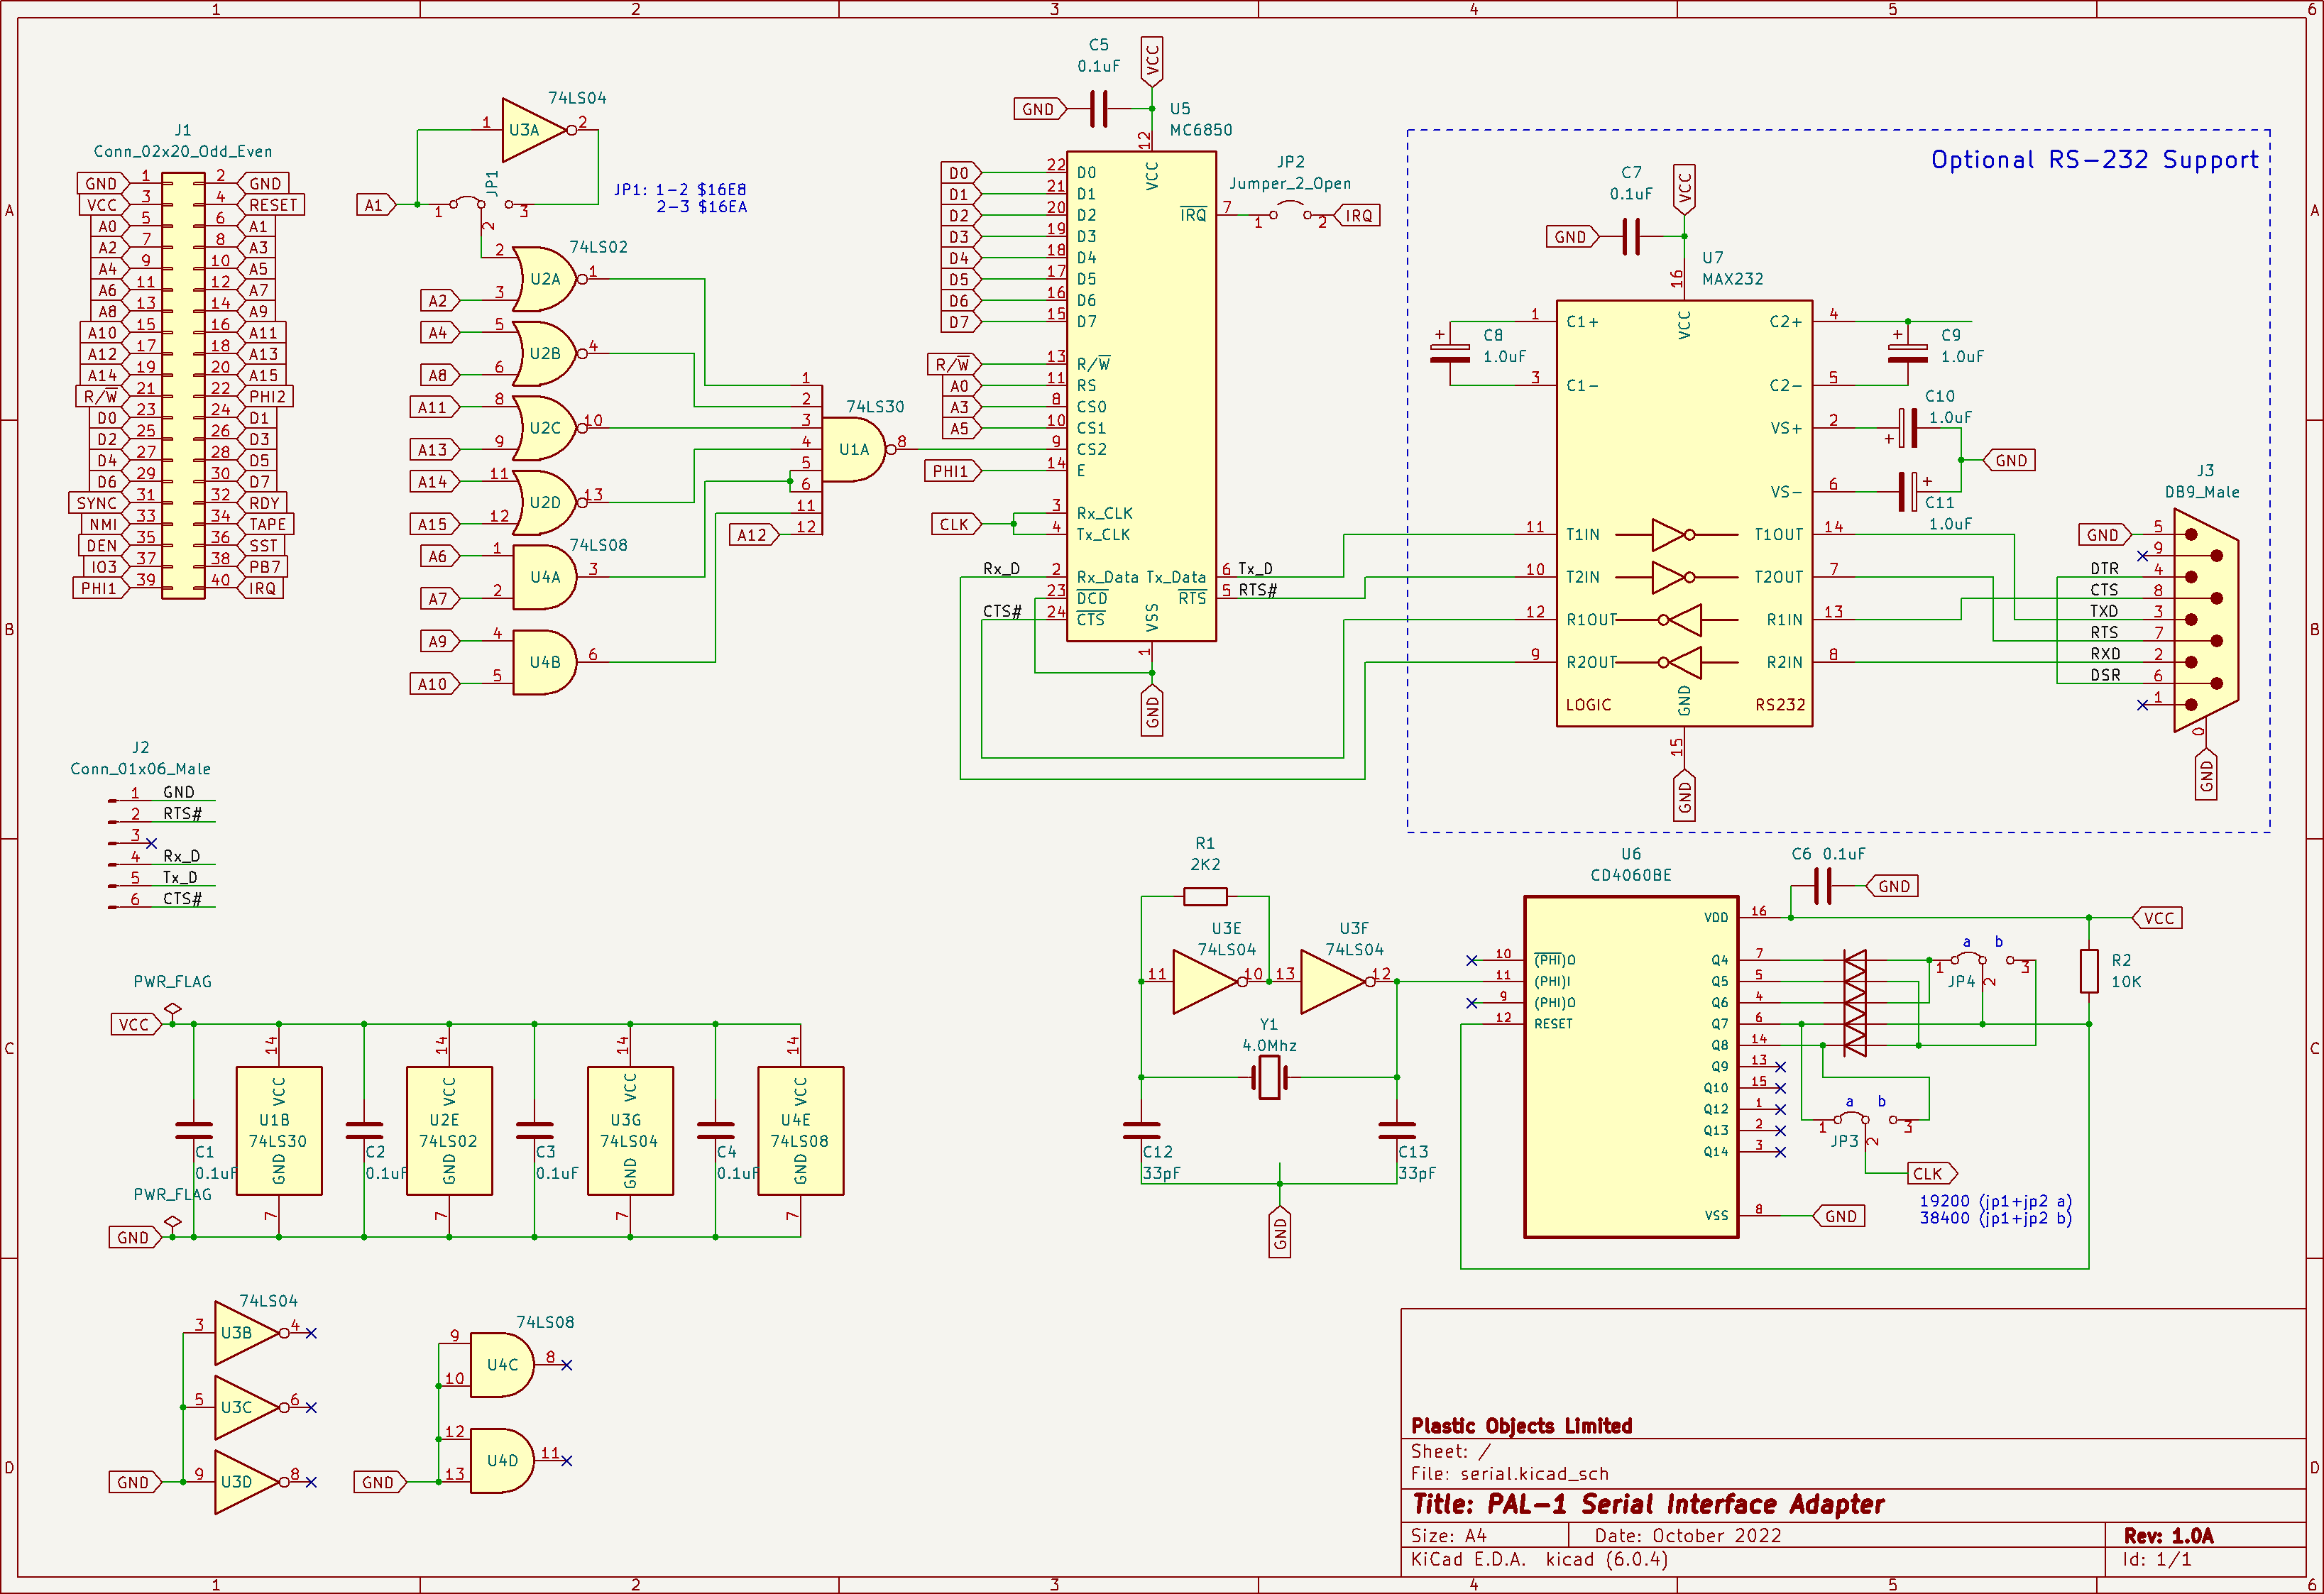
\includegraphics[width=1.8\textwidth,angle=90]{figures/schematic-1.0a.png}
    }
\end{figure}
\end{document} 

\chapter{Board layout}
\begin{figure}[h!]
\centering

\includegraphics[scale=2]{figures/serial-brd-1.0a.png}
\end{figure}

\documentclass[a4paper,11pt]{article}
\usepackage[lmargin=142pt,rmargin=95pt,tmargin=127pt,bmargin=123pt]{geometry}
\usepackage[table]{xcolor}
\usepackage{csvsimple}
\usepackage{caption}
\newcommand{\chapter}{\section*}
\captionsetup[table]{labelformat=empty}
\begin{document}
\chapter{Bill of Materials}
\label{sec:bom}
\begin{table}[htb]
\csvreader[head to column names,
	tabular={| c | c | c | p{7cm} |},
	table head=\hline\rowcolor{gray!20}\textbf{Part} & \textbf{Qty} & \textbf{Value} & \textbf{Description}\\\hline,
	late after last line=\\\hline]{serial-bom-1.0a.csv}{}
	{\ref&\qty&\val&\component}  
\caption{PAL-1 Serial Interface Adapter v1.0A components}
\label{tab:bom}  
\end{table}
\end{document} 


\bibliography{serial}
\bibliographystyle{jox}
\addcontentsline{toc}{chapter}{References}

\end{document}